\documentclass{article}

\usepackage[a4paper,hmargin=1.2in,vmargin=1.5in]{geometry}
\usepackage[parfill]{parskip} % for distance between paragraphs
\usepackage{ragged2e} % for alignment
\usepackage{hyperref} % for link
\usepackage{fancyhdr} % for header, footer
\usepackage{xcolor}  % for color
\usepackage{graphicx} % for figure
\usepackage{floatrow} % for formatting figures
\usepackage{enumitem} % for adjusting list spacing 
\usepackage{amsmath} 
\usepackage{amsthm} 
\usepackage{amssymb} 
\usepackage{esint}

\newtheorem{theorem}{Theorem}
\newtheorem{lemma}{Lemma}
\newtheorem{corollary}[theorem]{Corollary}
\newtheorem{proposition}{Proposition}[section]
\theoremstyle{remark}
\newtheorem*{remark}{Remark}

\setlength{\parskip}{0.5em}

\pagestyle{fancy}
\fancyhf{}
\lhead{190050113-190050080-190020010}
\rhead{CS 215}
\cfoot{Page \thepage}
\renewcommand{\footrulewidth}{1pt}

\usepackage{titlesec}
\titleformat{\section}
  {\Large\bfseries}{}{1em}{}

\title{Assignment 1: CS 215}

\author{
  \textbf{190050113} Shivam Raj
  \and
  \textbf{190050080} Pawan Kumar
  \and
  \textbf{190020010} Aman Singh
}

\date{\today}

\begin{document}

\pagenumbering{gobble}
\maketitle
\tableofcontents

\newpage
\pagenumbering{arabic}

\section{Question 1}
\textbf{(a)} The situation is equivalent to distributing $n$ books to $n$ people. The total number of ways of doing that is $n!$. There is only 1 way in which everyone gets his book back. So the probability of it happening is $\boxed{1/n!}$ \par

\textbf{(b)} There is only 1 way of distributing $m$ books to their respective $m$ owners. And for this way there are $(n-m)!$ ways of distributing the left $n-m$ books among left $n-m$ people for a total of $1\,\text{x}\,(n-m)!=(n-m)!$ ways. So the probability of it happening is $\boxed{(n-m)!/n!}$ \par

\textbf{(c)} There are $m!$ way of distributing the $m$ books belonging to the last $m$ people to the first $m$ people. And for each such way there are $(n-m)!$ ways of distributing the left $n-m$ books among left $n-m$ people for a total of $m!\,\text{x}\,(n-m)!=m!(n-m)!$ ways. So the probability of it happening is $\boxed{m!(n-m)!/n!}$ \par

\textbf{(d)}

\section{Question 2}
\section{Question 3}
\section{Question 4}
\section{Question 5}
\hspace{2.5em} \textbf{(a)}.
\begin{center}
    \hspace{1.25em}$P(C_1|Z_1)= \frac{1}{3}$ \par
    \hspace{1.25em}$P(C_2|Z_1)=\frac{1}{3}$ \par
    \hspace{1.25em}$P(C_3|Z_1)=\frac{1}{3}$ \par
\end{center}

\hspace{2.5em} \textbf{(b)}
$P(H_3|C_1, Z_1)=\frac{1}{2}$ (if car is present behind first door so rest two doors have equal probability)\par
$P(H_3|C_2, Z_1)=1$ (if car is present behind door 2, so the host will always pick door 3) \par
$P(H_3|C_3, Z_1)=0$ (if  car is present behind door 3 , them host will never select it )\par


\hspace{2.5em} \textbf{(c)}
\begin {center}
$P(H_3|C_2, Z_1)=1 $ \par
$ P(C_2,Z_1)=P(C_2|Z_1) \times P(Z_1)=\frac{1}{3} \cdot \frac{1}{3}=\frac{1}{9}$\par
$ P(H_3|Z_1)= \frac{1}{3}\cdot\frac{1}{2}+\frac{1}{3}\cdot1+\frac{1}{3}\cdot0=\frac{1}{2} $ \par
\begin {align*}
P(H_3,Z_1) &= P(H_3|Z_1) \times P(Z_1) \\
&=\frac{1}{2} \cdot \frac{1}{3}\\
&= \frac{1}{6}
\end {align*}

\begin{align*}
    P(C_2|H_3,Z_1) & = \dfrac{P(H_3|C_2,Z_1)P(C_2,Z_1)}{P(H_3,Z_1)} \\
                   & = \dfrac{1 \times \frac{1}{9}}{\frac{1}{6}}    \\
                   & = \dfrac{2}{3}
\end{align*}


\end {center}

\hspace{2.5em} \textbf{(d)}
\begin{center}
    \begin{align*}
        P(C_1|H_3,Z_1) & = \dfrac{P(H_3|C_1,Z_1)P(C_1,Z_1)}{P(H_3,Z_1)}       \\
                       & =\dfrac{\frac{1}{2} \times \frac{1}{9}}{\frac{1}{6}} \\
                       & = \dfrac{1}{3}
    \end{align*}



\end{center}


\hspace{2.5em} \textbf{(e)}
$P(C_2|H_3,Z_1) > P(C_1|H_3,Z_1)$ \par
\hspace{3.0em}So, Switching will be beneficial \par

\hspace{2.5em} \textbf{(f)}
\begin{center}
    $ \forall_i P(H_3|C_i,Z_1)=\dfrac{1}{2}$ \par
    $\forall_i P(C_i,Z_1)=\dfrac{1}{3}$ \par

    $P(H_3|Z_1)=\dfrac{1}{2}$ \par
    $P(H_3,Z_1)=P(H_3|Z_1) \times P(Z_1)=\dfrac{1}{2} \cdot \dfrac{1}{3}=\dfrac{1}{6} $ \par
    \begin{align*}
        P(C_2|H_3,Z_1) & = \dfrac{P(H_3|C_2,Z_1)P(C_2,Z_1)}{P(H_3,Z_1)} \\
                       & = \dfrac{\frac{1}{2} \times \frac{1}{9}}{\frac{1}{6}}    \\
                       & = \dfrac{1}{3}
    \end{align*}
    \begin{align*}
        P(C_1|H_3,Z_1) & = \dfrac{P(H_3|C_1,Z_1)P(C_1,Z_1)}{P(H_3,Z_1)}       \\
                       & =\dfrac{\frac{1}{2} \times \frac{1}{9}}{\frac{1}{6}} \\
                       & = \dfrac{1}{3}
    \end{align*}

    $P(C_2|H_3,Z_1) = P(C_1|H_3,Z_1)$. So switching won't create any difference.
    


\end{center}





\newpage

\section{Question 6}

% graph bohot faaltu hai

\begin{center}
    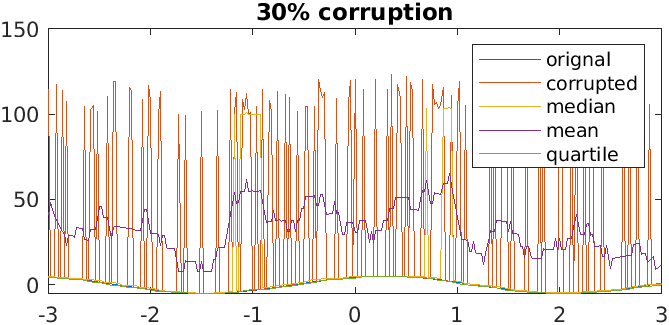
\includegraphics{q6(1).png}
    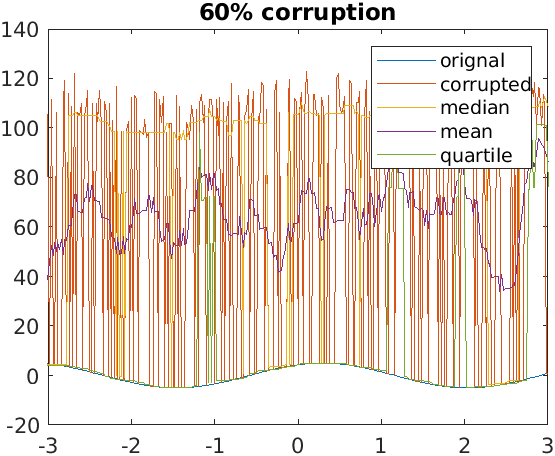
\includegraphics{q6(2).png}
\end{center}

\end{document}
